\part{Résultats et discussions}

\chapter{Une esthétique canonique multi-échelle}

Dans ce chapitre, nous présentons les résultats de nos différentes approches. Les hypothèses du mémoire semblent se vérifier statistiquement, et nous évaluons leur solidité statistique avec différentes métriques et différentes approches. 

\section{A l'échelle du roman}

Le modèle parvient à 75.3\% d'efficacité en validation croisée à l'échelle du roman. Dans notre cas de classification binaire, cela veut dire que la prédiction de la canonicité se révèle être bonne pour trois textes sur quatre. Il est admis que les résultats d'un modèle statistique sont fiables lorsque ses performances atteignent entre 75\% et 80\% d'efficacité, si les autres métriques du modèle convergent vers une stabilité autour de ces valeurs.

	\begin{table}[ht]
		\centering % Centre the table on the slide
		\begin{tabular}{l c c c c c}
			\toprule
    			 & precision & recall & f1-score & support & accuracy \\
			\toprule
			canon & 0.746 & 0.598 & 0.662 & 52 \\
			\midrule
			non-canon & 0.754 & 0.858 & 0.806 & 76\\
			\midrule
			full dataset & & & & 128 &\textbf{0.753} \\
			\midrule
			macro-average & 0.752 & 0.728 & 0.732 & 128\\
			\midrule
			weighted average & 0.751 & 0.751 & 0.746 & 128\\

			\bottomrule
		\end{tabular}
	\caption{Résultats de l'évaluation du modèle en validation croisée}
	\end{table} 
% see https://datascience.stackexchange.com/questions/86537/scikit-learn-classification-reports-f1-accuracy
Le modèle prédit mieux les ouvrages non-canoniques que les autres, mais le score de précision est plutôt bon (0.746). C'est le rappel (recall) qui pose des problèmes à notre modèle, c'est à dire que lorsqu'il prédit le label canonique il se trompe rarement, mais il n'arrive pas à le prédire dans un grand nombre de cas. Nous voyons là des signes du déséquilibre encore présent dans nos échantillons d'entraînement. 

Pour renforcer les résultats, nous entreprenons une démarche aléatoire pour nous assurer que le modèle statistique détecte bien des différences textuelles associées à nos méta-données plutôt que d'arriver artificiellement à séparer les deux classes. Cette approche aléatoire se réalise assez facilement, en désignant une classe canon ou non canon aléatoirement pour tous nos romans. Les résultats oscillent entre 45\% et 55\% d'efficacité, ce qui montre bien que le SVM n'arrive pas à séparer artificiellement nos deux classes sans raisons textuelles latentes. Ainsi, il se passe véritablement quelque chose dans les ouvrages canoniques. Nous désignons par dialecte canonique ce résultat, dont nous discuterons dans la suite du mémoire. 

\bigskip
\begin{figure}[!ht]
    \centering
    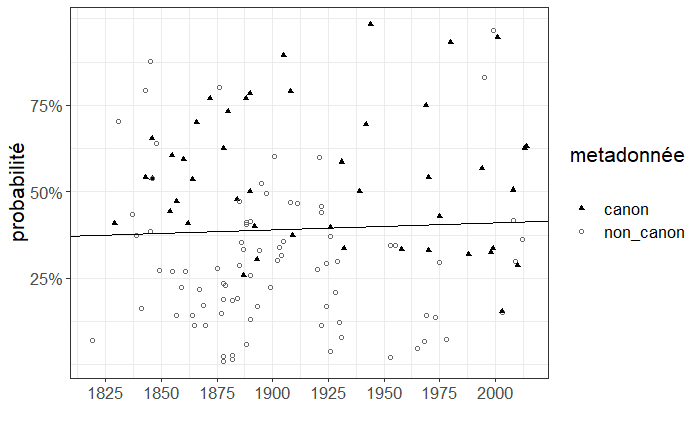
\includegraphics[width=15cm]{img/08_main_vis_svm.png}
    \caption{Probabilité prédite d'appartenir au canon littéraire, canon des romans}
    \label{svm_novel}
\end{figure}

Dans la figure \ref{svm_novel}\footnote{Nous reproduisons ici la visualisation de Ted Undewood dans son livre \cite{underwood_distant_2019}, page 80, voir \cite{underwood_tedunderwoodhorizon_2018} pour le code} nous projetons la probabilité prédite de chaque roman à appartenir au canon littéraire. Tous ces romans proviennent de l'échantillon de test, sur lequel on évalue la performance de généralisation du modèle. Les triangles représentent les romans classés comme canoniques et les cercles ceux non-canoniques. Le SVM arrive assez bien à détecter les deux classes, peu de romans canoniques sont classés non-canoniques, à l'exception de la fin du XX\ieme siècle, où le modèle fait quelques erreurs. La droite correspond à une régression linéaire de l'ensemble des probabilités canoniques assignées à chaque roman par notre modèle. Nous constatons ainsi une légère hausse de cette probabilité au cours du temps et nous commenterons ce résultat qui se renforce à l'échelle des auteurs.


\section{A l'échelle de l'auteur}

Le modèle atteint 90.4\% d'efficacité en validation croisée à l'échelle de l'auteur. Les résultats sont ainsi nettement meilleurs qu'à l'échelle des romans. 
	\begin{table}[ht]
		\centering % Centre the table on the slide
		\begin{tabular}{l c c c c c}
			\toprule
    			 & precision & recall & f1-score & support & accuracy \\
			\toprule
			canon & 0.866 & 0.888 & 0.878 & 231 \\
			\midrule
			non-canon & 0.928 & 0.911 & 0.921 & 361 \\
			\midrule
			full dataset & & & & 592 & \textbf{0.904}\\
			\midrule
			macro-average & 0.898 & 0.902 & 0.898 & 592 \\
			\midrule
			weighted average & 0.904 & 0.904 & 0.904 & 592 \\

			\bottomrule
		\end{tabular}
	\caption{Résultats de l'évaluation du modèle en validation croisée}
	\end{table} 

\bigskip
\begin{figure}[!ht]
    \centering
    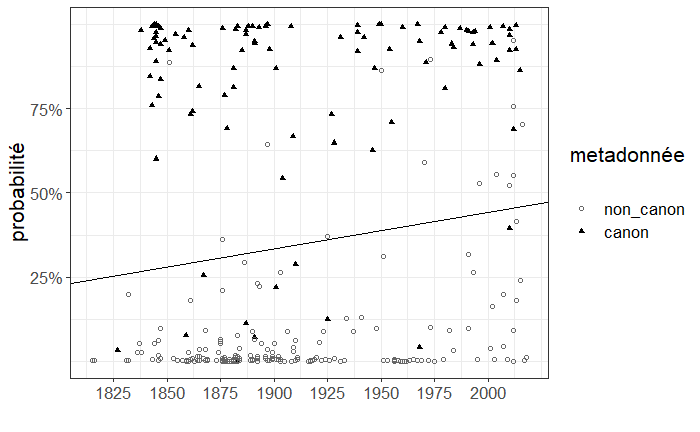
\includegraphics[width=15cm]{img/09_fabula_visual_svm.png}
    \caption{Probabilité prédite d'appartenir au canon littéraire, canon des auteurs}
    \label{svm_author}
\end{figure}


Dans la figure \ref{svm_author} nous projetons de la même manière la probabilité prédite de chaque roman à appartenir au canon littéraire, avec les méta-données canoniques à l'échelle de l'auteur. On remarque que le SVM est bien meilleur à cette échelle, c'est à dire bien plus confiant dans ses prédictions qu'à l'échelle des romans. Les deux groupes sont très distincts sur la figure \ref{svm_author}, et les erreurs sont moins nombreuses.   


Au regard de ces résultats, nous nous sommes demandés si le modèle ne détectait pas des indices linguistiques d'un groupe d'auteurs. 

Nous voulions savoir si le modèle ne reconnaissait pas l'idiolecte des auteurs canoniques sur lequel il s'était entraîné présents dans les œuvres de l'échantillon test. Si cela se vérifiait, notre modèle serait capable de réaliser des attributions d'auteurs et non de détecter un dialecte canonique. 

Ainsi nous avons entrepris de créer des jeux de données ne comportant qu'un roman par auteur pour exclure la probabilité que le modèle ne reconnaisse les ouvrages canoniques par la signature textuelle de leur auteur. Les résultats de cette démarche gardent une très bonne stabilité, c'est à dire que le modèle détecte bien quelque chose sans relation explicite avec les auteurs. 

Une des raisons qui pourraient expliquer la différence dans les performances entre les deux échelles de canonicité serait la taille de l'échantillon sur lequel le modèle est entraîné. En effet un défaut du SVM est de favoriser la classe la plus importante du jeu de données. Notre canon littéraire, à l'échelle du roman, n'est constitué que de 264 éléments, et même avec des procédures d'apprentissage non-équilibrées, il faut faire attention à la répartition des classes dans le jeu de donnée de l'échantillon d'entraînement. Ainsi, nous avons mis en place un ratio de répartition d'au moins 35\% de romans canoniques et 65\% de non canoniques au maximum. Le problème est que lorsque l'on travaille avec l'indice de canonicité à l'échelle des romans, la taille de l'échantillon de travail est moins important que celui à l'échelle des auteurs, de l'ordre de 800 éléments pour l'échelle de canonicité des romans et tout le corpus (3000 romans) à l'échelle des auteurs. De nombreux auteurs considérés comme canoniques ont beaucoup écrit d'ouvrages, cela explique la grande différence entre nos deux approches. Avec ce ratio et des procédures implémentées grâce à la librairie python imblearn\footnote{https://imbalanced-learn.org/stable/index.html}, le modèle fait des progrès de l'ordre de 5\% d'efficacité.

La régression linéaire projetée sur le graphe témoigne d'une tendance globale détectée par notre modèle. La probabilité d'appartenir au canon littéraire augmente avec le temps. Techniquement, cette hausse est une erreur. Les romans ne sont pas plus susceptibles d'appartenir au canon littéraire parce qu'ils sont publiés plus tard. Mais cela veut dire que le modèle échoue à produire des critères valides pour deux siècles de production littéraire. Les livres publiés plus tard comportent plus de signes linguistiques associés au canon littéraire. On remarque qu'une majorité des erreurs du modèle se trouvent entre les années 1975 jusqu'à nos jours. Des romans non canoniques (dont l'auteur n'est pas considéré comme canonique), obtiennent un bon score de canonicité. Le modèle perd en assurance et de nombreux romans se trouvent dans un entre-deux. On pourrait expliquer cela par une usure de la norme canonique, qui n'est plus aussi facile à discerner depuis les années 1975, malgré une distinction très forte durant 150 ans. 

En plus de ces hypothèses, on pourrait invoquer les limites de l'expérience pour expliquer cette tendance. En effet, on remarque que beaucoup de données tests se situent dans la deuxième partie du XIX\ieme siècle, où par ailleurs le modèle est très performant. C'est peut-être un biais du corpus que nous avons là, puisque cette période est proportionnellement très représentée dans notre corpus, comme on peut le constater en figure \ref{corpus_bar}. Le modèle a plus de données d'entraînement sur cette période, donc il se spécialise dessus. Pour autant, ce sur-apprentissage ne semble pas rédhibitoire puisque les données sont très bonnes sur les autres périodes aussi. Cela témoigne plutôt de la stabilité de la norme esthétique, puisque notre modèle repose en partie sur un léger sur-apprentissage des données plus nombreuses de la deuxième partie du XIX\ieme siècle, mais est capable de généraliser sur la longue durée.


\chapter{Discussions}

\section{Étude des cas limites}

L'étude des erreurs les plus importantes de nos modèles peut dire beaucoup de la manière dont ils se comportent. 

\begin{figure}[!ht]
    \centering
    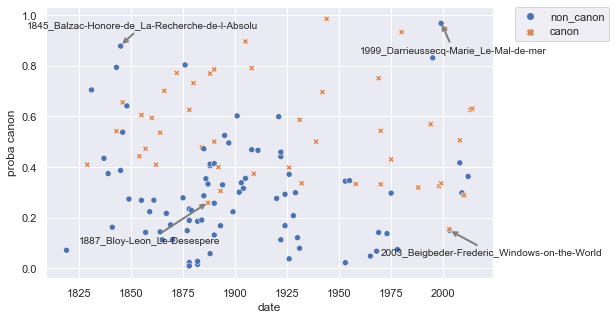
\includegraphics[width=15cm]{img/10_outliers_main_results.png}
    \caption{Cas limites du modèle entraîné à l'échelle des romans}
    \label{outlier_novel}
\end{figure}

La figure \ref{outlier_novel} met en avant quatre erreurs du modèle. Nous rappelons qu'à cette échelle le modèle performe à 75\% d'efficacité, donc les erreurs sont assez nombreuses. La canonicité prédite du roman de Balzac \textit{La recherche de l'absolu} est très importante, avec près de 90\% de probabilité. Pourtant, ce roman ne fait pas partie de notre canon littéraire. Ce roman de Balzac est classé dans les Études philosophiques de La Comédie humaine. Pour notre modèle, ce roman remplit tous les critères linguistiques relatifs au canon littéraire. Il en va de même pour le roman de Marie Darrieussecq, \textit{Le mal de mer}, qui pourtant est publié 150 années plus tard. Ce dernier n'est pas particulièrement resté dans les mémoires, du moins il n'est pas rentré dans un processus de canonisation. Pourtant, notre modèle le détecte comme tel. Cela peut re-légitimer cette œuvre, qui, au moins dans son contenu linguistique, fait aussi bien que les grands classiques de la littérature française. On constate d'autres erreurs du modèle dans le sens inverse. Des textes appartenant à notre canon littéraire ne sont pas bien notés par le modèle statistique. Par exemple, \textit{Windows on the world}, de Frédéric Beigbeder, fait parti de notre canon puisqu'il a gagné le prix Interallié en 2003. Ce roman relate les dernières minutes des victimes des attaques du World Trade Center le 11 septembre 2001. On constate ici les limites de nos méta-données, puisque le roman en question a pour vocation de raconter une histoire qui puisse toucher beaucoup de gens, en les amenant sur un sujet qui a bouleversé la société, plus que celle de rentrer dans le canon littéraire. \textit{Le désespéré}, est le premier roman de Léon Bloy, publié en 1887. Ce roman est canonique parce qu'il a été republié dans la collection \textit{Littérature Classique} de Garnier Flammarion en 2010. Il n'est pas aisé de comprendre pourquoi ce roman ne correspond pas à l'esthétique canonique perçue par notre modèle. Pour autant, la singularité de cette œuvre a été soulignée par Pierre Glaudes dans l'appareil critique de la réédition : \enquote{\textit{Le désespéré} est surtout un aérolithe littéraire, écrit dans une langue barbelée de mots rares, étrangement mystique, une œuvre d'une surprenante modernité}. Il semble que notre modèle donne raison à Pierre Glaudes, le roman sort des conventions et de l'esthétique du canon littéraire. 


A l'échelle des auteurs, le modèle est bien plus performant, mais quelques erreurs restent à noter comme on peut le voir en figure \ref{outlier_author}. 
\begin{figure}[!ht]
    \centering
    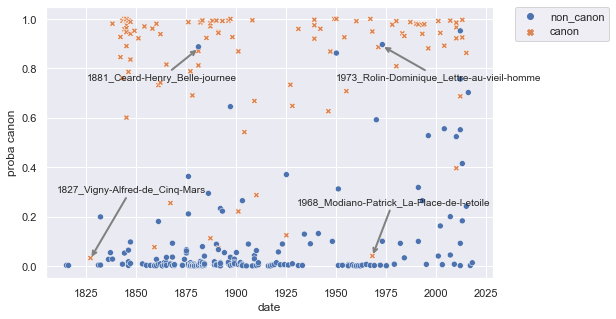
\includegraphics[width=15cm]{img/11_outliers_fabula_results.png}
    \caption{Cas limites du modèle entraîné à l'échelle des auteurs}
    \label{outlier_author}
\end{figure}

On a par exemple la \textit{Belle journée} d'Henry Céard qui est très bien noté par le modèle. Paru en 1881, ce roman est une ré-interprétation de \textit{Madame Bovary}, en forme d'hommage à Flaubert, mort un an auparavant. Henry Céard est un disciple de Flaubert et de Zola, son style se rapproche de ces derniers, même si l'histoire littéraire n'a pas retenu cet auteur. On peut donc expliquer cette erreur par la démarche même du roman qui est une imitation du style et du thème du roman de Flaubert. De la même manière, le livre de Dominique Rolin \textit{Lettre au vieil homme}, publié en 1973 est perçu comme canonique par le modèle, alors que l'écrivaine n'est pas retenue dans notre canon littéraire.

Au contraire, le roman \textit{Cinq mars}, d'Alfred de Vigny, est dans notre canon mais n'est pas admis comme tel par le modèle. Ce roman est considéré comme le premier roman historique, et l'on peut émettre l'hypothèse que c'est en cela qu'il se démarque de la manière commune de faire des romans pour notre modèle statistique. Enfin, le roman de Patrick Modiano \textit{La place de l'étoile}, publié en en 1968 aux éditions Gallimard est lui aussi très mal noté par le modèle. Le registre parodique du roman semble expliquer le fait qu'il n'ait pas sa place dans le canon littéraire perçu par le modèle.

%A l'échelle d'un auteur ? Flaubert ou Maupassant par ex ?


\section{Caractéristiques discriminantes du modèle statistique}

Il faudrait maintenant comprendre comment nos modèles statistiques sont capables de prédire la canonicité. Un des intérêts de l'apprentissage machine est d'ailleurs la possibilité de plonger dans les inférences réalisées par le modèle. En effet, on peut récupérer les coefficients que le modèle assigne à chaque caractéristique pour séparer nos deux groupes. Dans la figure \ref{coefs}, nous projetons les 40 caractéristiques les plus discriminantes pour le modèle. En bleu, nous avons les 20 caractéristiques qui donnent le plus de poids à l'esthétique canonique, et en rouge celle non-canonique. 

%ted underwood p 81


\bigskip
\begin{figure}[!ht]
    \centering
    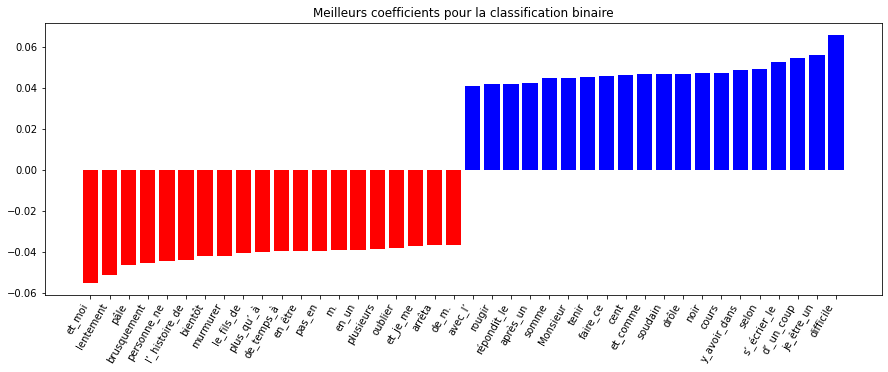
\includegraphics[width=17cm]{img/12_coef_fabula.png}
    \caption{coefficients discriminants pour le modèle, canon des auteurs}
    \label{coefs}
\end{figure}


Il est difficile d'appréhender ce qui se joue dans ces coefficients. Les mots \textit{difficile}, \textit{drôle} ou \textit{rougir} sont considérés plus canoniques que les mots \textit{pâle}, \textit{oublier} ou \textit{murmurer}. Le problème interprétatif auquel nous faisons face n'est pas dû à l'apprentissage machine mais plutôt à la complexité du phénomène que nous modélisons, la réception littéraire. Il est compliqué d'attribuer la canonicité à un groupe de mots précis, et comme nous avons fondé notre travail sur une approche linguistique avec des mots outils, nous avons en plus à interpréter des mots très courants. 

Pour comprendre ce que le modèle détecte, nous représentons dans le texte les coefficients de ce dernier. Les 500 caractéristiques les plus canoniques sont coloriés en bleu, les 500 les plus non-canoniques en rouge et le reste n'est pas représenté. Nous projetons en figure \ref{extrait_colette} ces coefficients sur un extrait de \textit{Sido}, roman écrit par Colette et publié en 1929.

\bigskip
\begin{figure}[!ht]
    \centering
    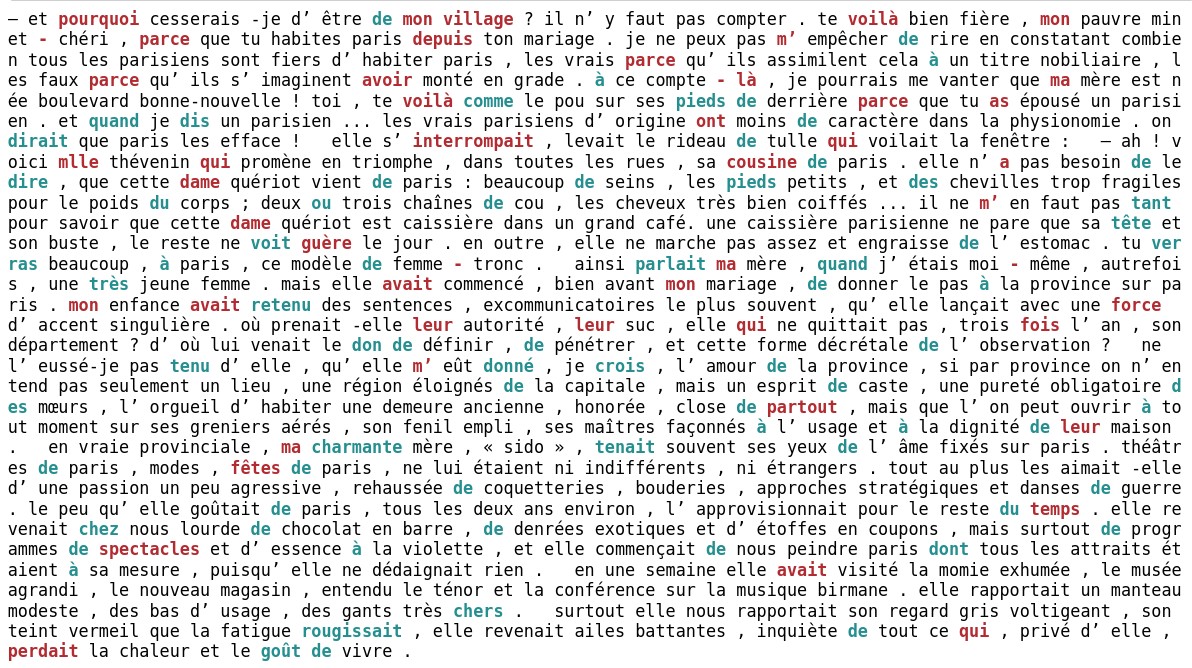
\includegraphics[width=18cm]{img/13_sido_colored.png}
    \label{extrait_colette}
    \caption{Extrait de Sido, écrit par Colette, canonicité coloriée}
\end{figure}

Dans cet extrait, nous voyons bien que le modèle ne détecte pas une manière d'être canonique. Colette écrit avec des mots considérés comme non-canonique par le modèle, comme les pronoms possessifs \textit{mon} ou \textit{ma}. Le crible du modèle statistique révèle un ensemble de traits linguistiques spécifique mais pas exclusif à ces œuvres canoniques. Le verbe \textit{rougir} ou l'adjectif qualificatif \textit{charmante} en fin d'extrait ne sont pas uniquement dédiés aux auteurs canoniques, mais le choix de ces mots est d'avantage réalisé par ces derniers.


\section{Des motifs stylistiques}

Pour palier ce problème interprétatif, nous avons revu notre démarche, avec l'objectif de détecter plus d'éléments relatifs au style. Nous avons implémenté pour cela une approche similaire à la technique des motifs stylistiques. Selon, Dominique Legallois, Thierry Charnois et Meri Larjavaara, 
\begin{displayquote}\enquote{la caractérisation du style d'un auteur, peut bénéficier d'une nouvelle d'une nouvelle méthode en linguistique de corpus, la découverte de modèles séquentiels ou de \enquote{motifs}, c'est-à-dire des chaînes contiguës de formes de mots/lemmas/POS tag. L'analyse des motifs peut être considérée comme complémentaire aux approches discrètes}\footcite{legallois_balance_2018}.
\end{displayquote}

Dans cette section, les motifs ne vont pas nous servir à caractériser un style d'auteur, mais plutôt à spécifier l'esthétique canonique que nous détectons. Nous simplifions l'approche pour construire nos motifs. On récupère de la même manière des uni-grammes, bi-grammes et tri-grammes, avec cette fois ci l'étiquetage morpho-syntaxique des mots-outils et le lemme des autres mots. 
Nous mettons le tableau des scores en annexe \ref{perf_motif}. Les résultats sont sensiblement similaires à notre première approche, ce qui s'explique par la proximité des caractéristiques textuelles utilisées. Ces résultats semblent toutefois renforcer notre première intuition : il y a bien une esthétique particulière sélectionnée dans le canon littéraire construit par nos soins. 

\bigskip
\begin{figure}[!ht]
    \centering
    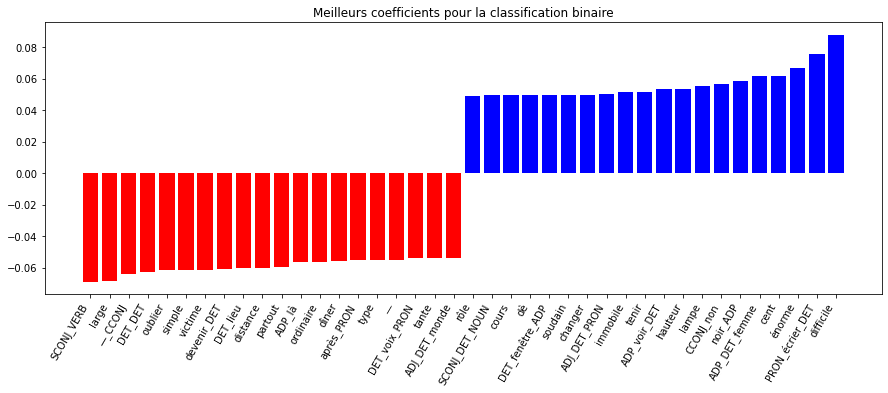
\includegraphics[width=17cm]{img/14_coefs_motifs.png}
    \caption{coefficients discriminant pour le modèle des motifs, canon des auteurs}
    \label{coefs_motifs}
\end{figure}

Dans la figure \ref{coefs_motifs} nous projetons les coefficients discriminants. On voit bien qu'en plus de mots simples, le modèle assigne de bons scores à des manières de construire une phrase. Le bi-gramme SCONJ\_VERB est la concaténation de deux mots consécutifs, en l'occurrence une conjonction de coordination avec un verbe, par exemple \enquote{Il n'est pas heureux, \textit{parce qu'habiter} en province n'est pas dans son intérêt}. Cette forme se rapproche plus selon le modèle d'une écriture non-canonique. Au contraire, le tri-gramme PRON\_écrier\_DET, qui donne par exemple\enquote{s'écria le personnage}, avec la forme pronominale du verbe écrier, est plus proche d'une écriture canonique. C'est une manière d'introduire du discours direct dans le récit, l'on ne peut pas conclure d'une utilisation plus prononcé du discours direct dans les romans canoniques avec cet unique indice.

\section{Test sur des données hors domaine d'étude}

Pour comprendre un peu mieux ce que le modèle détecte concrètement, nous lui avons donné des textes hors de son domaine d'étude pour voir quel score leur était attribué. En effet le modèle peut donner un score à tout texte écrit, même si ce n'est pas un texte littéraire. Il nous fallait des textes assez conséquents en terme de longueur, pour éviter d'avoir une matrice d'entraînement trop vide. Nous lui avons présenté deux différents textes : 

\begin{itemize}
    \item La page wikipédia du théorème de Bayes.\footnote{\url{https://fr.wikipedia.org/wiki/Théorème_de_Bayes}}
    \item Un extrait du Code Civil, le chapitre 2 du titre 2 du livre II.\footnote{\url{https://www.legifrance.gouv.fr/codes/texte_lc/LEGITEXT000006070721}}
\end{itemize}

Ce sont deux textes très formels, le premier présente une vulgarisation scientifique d'un théorème mathématique, avec une histoire et une contextualisation du théorème. L'autre comporte un chapitre du Code Civil, le tout représentant 8 articles avec de nombreux alinéas. En terme de longueur, les deux textes sont assimilables à des nouvelles suffisamment longues pour être modélisées correctement. Voici les résultats :
\bigskip

\begin{table}[ht]
    \centering
    \begin{tabular}{lrrl}
    \toprule
    {} &  proba canon &  proba non-canon & prediction \\
                     &              &                  &            \\
    \midrule
    Article du Théorème de Bayes  &         0.375779 &         0.624221 &  non\_canon \\
    Code Civil                &         0.454353 &         0.545647 &  non\_canon \\
    \bottomrule
    \end{tabular}
    \caption{Résultats des expérimentations hors domaine, canon des œuvres.}
\end{table}

Le modèle reposant sur le canon des œuvres réagit assez bien à ce test, dans le sens où il n'a l'air de reconnaître ni les traits canoniques ni ceux non-canoniques. Si les deux sont classés \enquote{non-canon}, la probabilité d'appartenance montre que le modèle n'est pas vraiment sûr de lui. Le fait que ces deux énoncés très formels soient classés comme non-canon pourrait soutenir l'idée d'un style plus développé dans le canon littéraire. 


\begin{table}[ht]
    \centering
    \begin{tabular}{lrrl}
    \toprule
    {} &  proba canon & proba non-canon &    prediction \\
                     &                  &              &             \\
    \midrule
    Article du Théorème de Bayes  &      0.484885  &    0.515115  &    non\_canon \\
    Code Civil                &      0.580976  &    0.419024  &         canon \\
    \bottomrule

    \end{tabular}
    \caption{Résultats des expérimentations hors domaine, canon des auteurs}
\end{table}

Le modèle reposant sur le canon des auteurs est lui aussi dubitatif quand à ces textes et ne sait pas comment les classer. A cette échelle le modèle se montrait très sûr de lui, et très peu de scores étaient entre 0.8 et 0.2. Cela montre bien que ces deux textes ne ressemblent en rien aux traits canoniques ou non-canoniques.

\newpage

\section{Sélectivité canonique dans la production d'un auteur}

Nos modèles détectent une filtration linguistique d'une certaine manière d'écrire des romans. Cette sélection ne se fait pas seulement au niveaux des auteurs, que l'on considère comme classique ou non, mais aussi au sein de la production littéraire d'un même auteur. Nous présentons ici les résultats des expériences menées à partir des romans de Colette, Georges Perec et Guy de Maupassant.

Pour mieux comprendre ce qui se joue à cette échelle, nous avons mis en place d'autres expériences. Avec des réductions de dimension, et plus précisément des analyses en composantes principales (ACP), nous projetons tous les ouvrages d'un même auteur sur un seul plan pour pouvoir comparer les ouvrages entre eux. 

L’ACP est une méthode bien connue de réduction de dimension qui va permettre de visualiser des données complexes pour y discerner des regroupements, des typologies. L'ACP entraîne une perte d'information car les dimensions sont réduites, mais les informations conservées sont sensées être les plus significatives.

\subsection{Colette}

\bigskip
\begin{figure}[!ht]
    \centering
    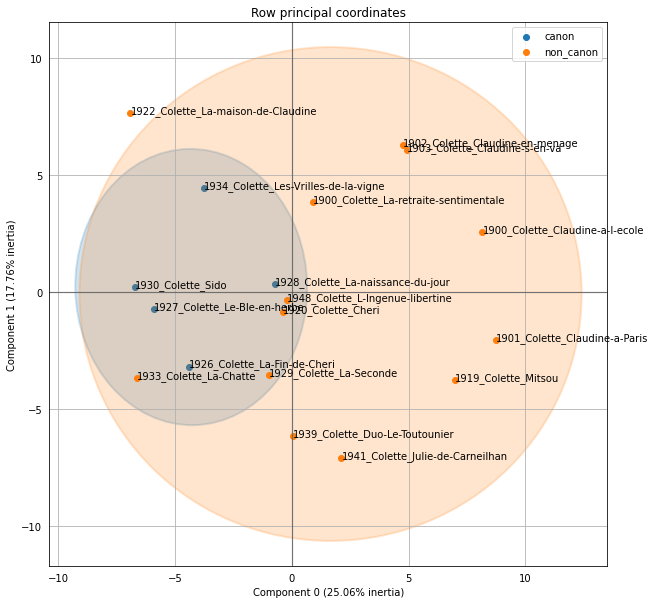
\includegraphics[width=11cm]{img/15_pca_Colette.png}
    \caption{Sélectivité canonique chez Colette}
    \label{colette}
\end{figure}

Nous avons réalisé des réductions de dimension en figure \ref{colette} sur les écrits de Colette, une écrivaine célèbre du début du XX\ieme siècle. 

Deux éléments sont mis en avant dans ce graphique, d'une part en orange les romans de Colette non-canoniques, et d'autre part en bleu les ouvrages considérés comme canoniques. On remarque que ces derniers forment un groupe assez distinct au sein de la production littéraire de Colette. L'ACP appose naturellement les romans canoniques dans la même partie du graphique, c'est à dire qu'il y a des similarités conséquentes entre ces romans. Les cinq romans canoniques sont tous écrits entre 1926 et 1934, ce qui pourrait expliquer la présence de ce groupe en tant qu'il correspond à un moment littéraire précis dans la vie de l'auteur. Loin de ce groupe se trouve la série des \textit{Claudine}, qui ont été des ouvrages très populaires mais pas intégré dans le canon. Ces ouvrages ont fait la popularité de l'auteur au début de sa carrière, mais ne correspondaient pas aux critères de sélection du canon. 


\subsection{Georges Perec}

Georges Perec est un écrivain qui a publié la majorité de ses œuvres dans la deuxième partie du XX\ieme siècle. Notre canon a retenu deux de ses ouvrages, \textit{Les choses}, publié en 1965 et \textit{La vie mode d'emploi}, publié en 1978.

\bigskip
\begin{figure}[!ht]
    \centering
    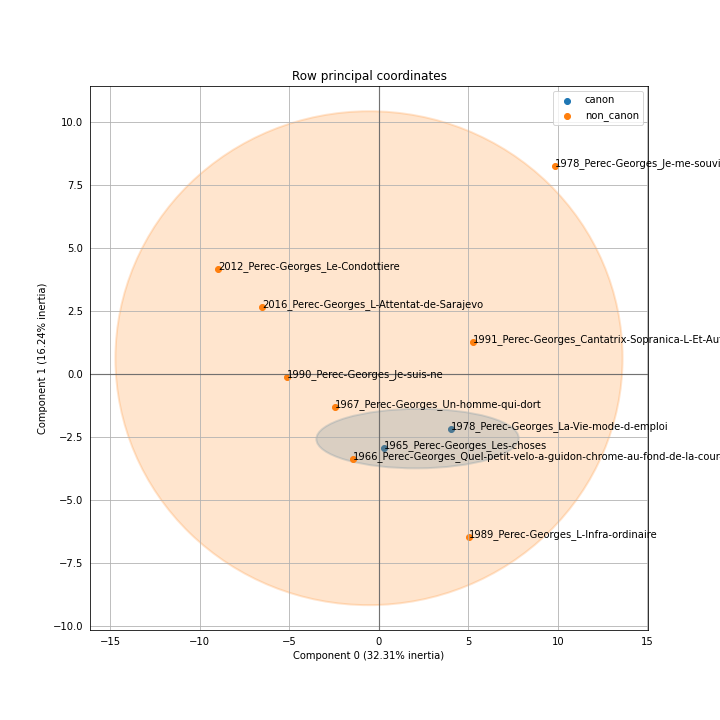
\includegraphics[width=11cm]{img/16_pca_Perec.png}
    \caption{Sélectivité canonique chez Georges Perec}
    \label{perec}
\end{figure}

L'ACP en figure \ref{perec} montre bien que ces deux ouvrages sont très similaires dans leur contenu, malgré le fait qu'ils aient été publiés à 13 années d'intervalle. Les romans acceptés dans le canon par la réception correspondent donc bien à une esthétique particulière, au sein même de la production d'un écrivain.

On remarquera que le roman \textit{Je me souviens} est très loin des autres romans, à cause de son caractère stylistiquement subversif. Le roman est un enchaînement de souvenirs de l'auteur, avec une anaphore \enquote{Je me souviens} sur tout le roman. 
C'est un roman qui a marqué la période mais il n'est pas rentré dans les critères de notre canon. 


\subsection{Guy de Maupassant}

Il est important de souligner que cette expérience ne marche pas pour tous nos auteurs. Examinons l'exemple des ouvrages de Guy de Maupassant, en figure \ref{maupa} : ce dernier est un auteur très productif, et la visualisation de la réduction de dimensionnalité ne parvient pas à séparer les canons des non-canons.

\bigskip
\begin{figure}[!ht]
    \centering
    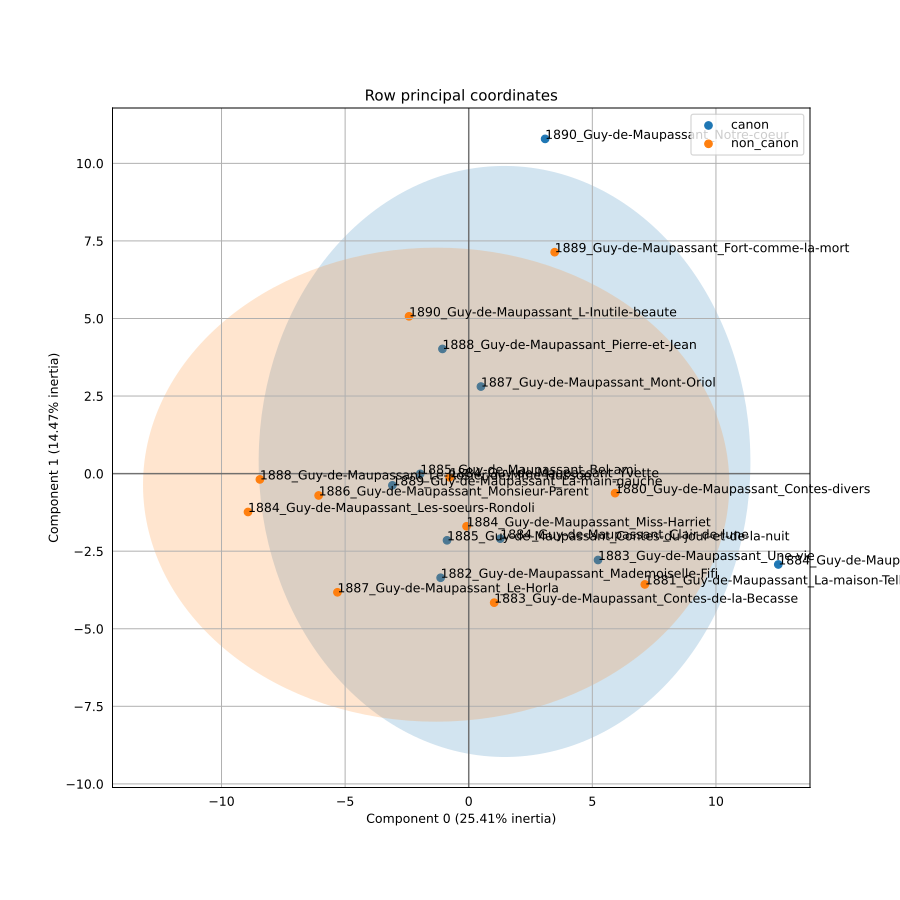
\includegraphics[width=11cm]{img/17_pca_Maupassant.png}
    \caption{Sélectivité canonique chez Maupassant}
    \label{maupa}
\end{figure}

Il y a une superposition des deux ensembles des œuvres, canoniques et non-canoniques. La critique et surtout l'institution scolaire ont tellement sacralisé le style de cet auteur que la distinction entre leurs œuvres de premier et de second plan ne tient plus, comme si le tamis sélectif avait fini par accepter la manière d'écrire de cet écrivain dans son ensemble, peu importe ses ouvrages. 

Ainsi, l'esthétique canonique constatée à l'échelle de milliers de romans par nos modèles statistiques semble sortir renforcée de nos différents tests et entrées de compréhension des données du modèle. L'étude des cas limites et les tests hors domaine d'étude semblent montrer la solidité du modèle ainsi que sa capacité à généraliser. Cette sélectivité du canon littéraire se constate aussi à l'échelle de la production d'un auteur, et ce malgré sa qualité de classique. Nos ACP montrent la filtration d'un certain type de contenu dans la production littéraire, entre un contenu conservé dans la mémoire collective et un autre laissé à l'abandon littéraire. 